\documentclass[12pt]{article}

\usepackage[english]{babel}
\usepackage[utf8]{inputenc}
\usepackage{fancyhdr}

\usepackage[margin=1in]{geometry}
\usepackage{pgf}
\usepackage{pgfplots}
\usepackage{siunitx}
\usepackage{tikz}
\usepackage{float}
\usepackage{amsmath}
\usepackage{enumitem}
\usepackage{textcomp}

\usepackage[font=small,labelfont=bf]{caption}
\usepackage[nodisplayskipstretch]{setspace}

\usetikzlibrary{scopes}
\usetikzlibrary{angles,quotes}
\usetikzlibrary{calc}
\graphicspath{ {/} }
\pgfplotsset{compat=1.5}

\newcommand*{\I}{\imath}
\newcommand*{\J}{\jmath}
\newcommand{\norm}[1]{\lvert #1 \rvert}

\setlist[enumerate, 1]{label=\alph*.}

\begin{document}
\sisetup{per-mode=symbol}

\begin{titlepage}
    \begin{center}
        \vspace*{1cm}
        \textbf{Electric Circuits 2}

        \vspace{0.5cm}
        Lab: 02

        \vspace{1cm}

        \textbf{Jaden Moore}

        \vfill

        Orange Coast College\\
        Physics A285L\\
        December 7th, 2021

    \end{center}
\end{titlepage}

\pagestyle{fancy}
\fancyhf{}
\setlength{\headheight}{15pt}
\lhead{Electric Circuits 2}
\rhead{Lab: 02}
\cfoot{\thepage}

\section{Introduction}
In this lab, we attach a resistance $R_L$ across two end terminals of a circuit. We then analyze the behavior of the various electrical quantities across the resistor as resistance increases. We then prove Thévenin's theorem by creating Thévenin's equivalent circuit and comparing the electrical quantities with the original circuit quantities.
\begin{figure}[H]
    \begin{center}
        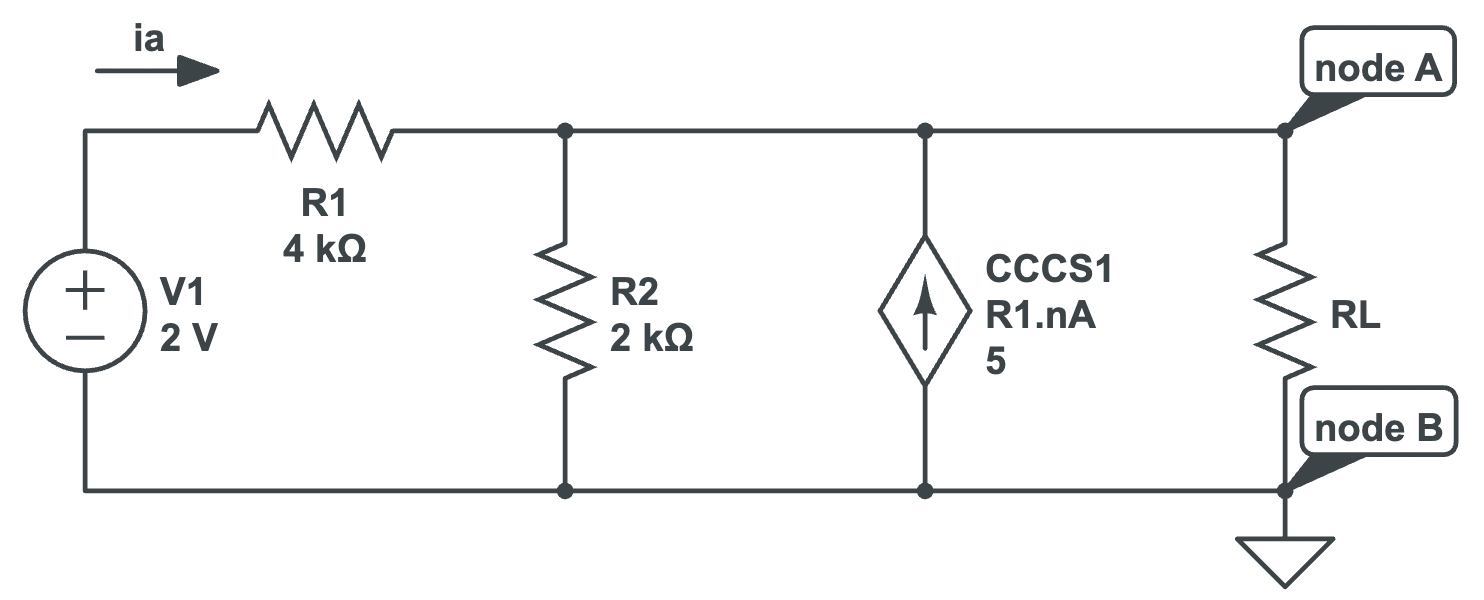
\includegraphics[scale=0.5]{circuit-1.png}
        \caption { Electric circuit with resistor $R_L$ across terminals A-B}
    \end{center}
\end{figure}
Consider the circuit presented in Figure (1). We place increasing resistances across $R_L$ and measure the current $i_L$, the voltage, $v_L$, and power $p_L$ across the resistor and record the data in the table below.

\newcolumntype{P}[1]{>{\centering\arraybackslash}p{#1}}

% \setlength{\tabcolsep}{4pt}
\renewcommand{\arraystretch}{1}

\begin{figure}[H]
    \begin{center}
        \begin{tabular}{ P{3cm} P{3cm} P{3cm} P{3cm} P{3cm} }
            \hline
            \multicolumn{5}{c}{Table 1: Recorded image and object distances from the lens}          \\

            \hline
            $R_L$ [$\Omega$] & $i_L$ [A] & $v_L$ [V] & $p_{L-exp}$	[W]          & $p_{L-theory}$ [W] \\
            \hline
            10               & 294.1E-05 & 0.029     & 086.5E-06	086.5052E-06
            56               & 269.8E-05 & 0.151     & 407.6E-06	407.5876E-06
            110              & 245.9E-05 & 0.27      & 001.025E-03	001.0246E-03
            180              & 220.6E-05 & 0.397     & 875.9E-06	875.8651E-06
            200              & 214.3E-05 & 0.429     & 918.4E-06	918.3673E-06
            270              & 194.8E-05 & 0.526     & 001.0E-03	001.0246E-03
            360              & 174.4E-05 & 0.628     & 001.1E-03	001.0952E-03
            430              & 161.3E-05 & 0.694     & 001.1E-03	001.1186E-03
            470              & 154.6E-05 & 0.727     & 112.4227E-05            & 112.3924E-05       \\
            560              & 141.5E-05 & 0.792     & 112.0755E-05            & 112.1396E-05       \\
            750              & 120.0E-05 & 0.9       & 108.0000E-05            & 108.0000E-05       \\
            1000             & 100.0E-05 & 1         & 100.0000E-05            & 100.0000E-05       \\
            1800             & 652.2E-06 & 1.174     & 765.6522E-06            & 765.5955E-06       \\
            2700             & 468.8E-06 & 1.266     & 593.4375E-06            & 593.2617E-06       \\
            3600             & 365.9E-06 & 1.317     & 481.8293E-06            & 481.8560E-06       \\
            5600             & 245.9E-06 & 1.377     & 338.6066E-06            & 338.6187E-06       \\
            27000            & 545.5E-07 & 1.473     & 803.4545E-07            & 803.3058E-07       \\
            110000           & 135.7E-07 & 1.493     & 202.6697E-07            & 202.6986E-07       \\
            220000           & 680.3E-08 & 1.497     & 101.8367E-07            & 101.8094E-07       \\
            750000           & 199.9E-08 & 1.499     & 299.6003E-08            & 299.6004E-08       \\
            1100000          & 136.3E-08 & 1.499     & 204.3162E-08            & 204.3596E-08       \\
            2400000          & 624.9E-09 & 1.5       & 937.3047E-09            & 937.1095E-09       \\
            4700000          & 319.1E-09 & 1.5       & 478.6725E-09            & 478.6216E-09       \\
            6200000          & 241.9E-09 & 1.5       & 362.8740E-09            & 362.8447E-09       \\
            8200000          & 182.9E-09 & 1.5       & 274.3735E-09            & 274.3568E-09       \\
            10000000         & 150.0E-09 & 1.5       & 224.9888E-09            & 224.9775E-09       \\
            \hline
        \end{tabular}
    \end{center}
\end{figure}

\begin{figure}[H]
    \centering
    \begin{tikzpicture}
        \pgfplotsset{width=10cm}
        \begin{axis}[
                xlabel={$R_L$ [$\Omega$]},
                ylabel={$i_L$ [A]},
                xmode=log,
                scaled y ticks=real:1e3,
                legend cell align = left,
                legend pos = north east,
                xtick pos=left,
                ytick pos=left
            ]
            \addplot[red, only marks, mark=o, smooth] table{CvR.txt};

            \addlegendimage{only marks}
            \addlegendentry{current $i_L$}
        \end{axis}
    \end{tikzpicture}
    \caption[12pt]{Current through load resistance $R_L$}
\end{figure}

\begin{figure}[H]
    \centering
    \begin{tikzpicture}
        \pgfplotsset{width=10cm}
        \begin{axis}[
                xlabel={$R_L$ [$\Omega$]},
                ylabel={$v_L$ [V]},
                xmode=log,
                scaled y ticks=real:1e3,
                legend cell align = left,
                legend pos = south east,
                xtick pos=left,
                ytick pos=left
            ]
            \addplot[blue, only marks, mark=o, smooth] table{VvR.txt};

            \addlegendimage{only marks}
            \addlegendentry{voltage $v_L$}
        \end{axis}
    \end{tikzpicture}
    \caption[12pt]{Voltage through load resistance $R_L$}
\end{figure}

\begin{figure}[H]
    \centering
    \begin{tikzpicture}
        \pgfplotsset{width=10cm,compat=1.3}
        \begin{axis}[
                xlabel={$R_L$ [$\Omega$]},
                ylabel={$i_L$ [A]},
                axis y line*=left,
                xmode=log,
                scaled y ticks=real:1e3,
            ]
            \addplot[red, only marks, mark=o, smooth] table{CvR.txt}; \label{plot_1}
        \end{axis}

        \begin{axis}[
                xlabel={$R_L$ [$\Omega$]},
                ylabel={$v_L$ [V]},
                xmode=log,
                hide x axis,
                axis y line*=right,
                legend cell align = left,
                legend style={at={(0.95,0.6)},anchor=north east}
            ]
            \addplot[blue, only marks, mark=o, smooth] table{VvR.txt}; \label{plot_2}

            \addlegendimage{/pgfplots/refstyle=plot_1}\addlegendentry{voltage $v_L$}
            \addlegendimage{/pgfplots/refstyle=plot_2}\addlegendentry{current $i_L$}
        \end{axis}

    \end{tikzpicture}
    \caption[12pt]{Current and voltage through load resistance $R_L$}
\end{figure}

\begin{figure}[H]
    \centering
    \begin{tikzpicture}
        \pgfplotsset{width=10cm}
        \begin{axis}[
                xlabel={$R_L$ [$\Omega$]},
                ylabel={$p_L$ [W]},
                xmode=log,
                scaled y ticks=real:1e3,
                legend cell align = left,
                legend pos = north east,
                xtick pos=left,
                ytick pos=left
            ]
            \addplot[orange, only marks, mark=o, smooth] table{PvR.txt};

            \addlegendimage{only marks}
            \addlegendentry{power $p_L$}
        \end{axis}
    \end{tikzpicture}
    \caption[12pt]{Power $p_L$ through load resistance $R_L$}
\end{figure}
\end{document}